\documentclass[../main/These_Mathias_Paget.tex]{subfiles}

%----------------------------------------------------------------------------------------
\begin{document}
%----------------------------------------------------------------------------------------
%2) Problème par programmation dynamique
%2.1) Problème 1D par DP
%2.2) Extension aux problèmes 2D
%2.3) Programmation Dynamique appliquée à la stéréo-reconstruction (SGM)
%2.4) SGM dans la taxonomie de la stéréo-reconstruction
%2.5) Variantes de la méthode
%3) Comparaison entre méthodes
%3.1) Réglage du coefficient de régularisation pour comparer des modèles
%3.2) Comparaison des méthodes par GC
%3.3) Comparaison SGM/GC

% macro tikz
%\draw[-] (\k) edge (\b);

\newcommand{\myimage}[3]{% blabla
\begin{tikzpicture}

% parameters
\def \W {#1}
\def \ST {#2}
\def \UJ {#3}

% styles
\tikzset{ActNode/.style={shape=circle,draw, fill=teal!40}}
\tikzset{ActNodea/.style={shape=circle,draw, fill=teal!50}}
\tikzset{ActNodeb/.style={shape=circle,draw, fill=teal!60}}

\tikzset{CenterNode/.style={shape=circle,draw, fill=red!70}}
\tikzset{AddLink/.style={color=red!70,line width=0.7 pt}}
\tikzset{BackFig/.style={color=black!50}}

\ifthenelse{\ST=1}{
	\pgfmathtruncatemacro{\UJ}{1}
}

\pgfmathsetmacro{\Winmax}{\W*2}
\pgfmathsetmacro{\Winlen}{\Winmax+1}

\foreach \i in {0,...,\Winmax}{
	\foreach \j in {0,...,\Winmax}{

		% / d f
		% b c e
		% g a k
	
		\pgfmathtruncatemacro{\k}{\i+\j*\Winlen}
		\pgfmathtruncatemacro{\a}{\k-1}
		\pgfmathtruncatemacro{\b}{\k-2-\Winlen}
		\pgfmathtruncatemacro{\c}{\k-1-\Winlen}
		\pgfmathtruncatemacro{\d}{\k-1-2*\Winlen}
		\pgfmathtruncatemacro{\e}{\k-\Winlen}
		\pgfmathtruncatemacro{\f}{\k-2*\Winlen}
		\pgfmathtruncatemacro{\g}{\k-2}
		
		\node (\k) at (\i/2,-\j/2) [circle,draw] {};
		
		\ifthenelse{\i>0}{
			\draw[-] (\k) edge[BackFig] (\a);
			
			\ifthenelse{\j>0}{
				\draw[-] (\k) edge[BackFig] (\e);
				
				\ifthenelse{\UJ=1}{
					\draw[-] (\k) edge[BackFig] (\c);
					\draw[-] (\a) edge[BackFig] (\e);
				}		
				
				\ifthenelse{\ST=1}{
					\ifthenelse{\i>1}{
						\draw[-] (\k) edge[BackFig] (\b);
						\draw[-] (\e) edge[BackFig] (\g);				
					}

					\ifthenelse{\j>1}{
						\draw[-] (\k) edge[BackFig] (\d);
						\draw[-] (\a) edge[BackFig] (\f);				
					}
				
				}
			}
		}
		{
			\ifthenelse{\j>0}{
				\draw[-] (\k) edge[BackFig] (\e);
			}
			
		}
		
	}
}



% inpaint
\foreach \l in {1,...,\W}{
	
	% n o p
	% q m r
	% s t u
	\pgfmathtruncatemacro{\m}{\W+\W*\Winlen}
	\pgfmathtruncatemacro{\z}{\l-1}
	
	\pgfmathtruncatemacro{\x}{\W-\l}
	\pgfmathtruncatemacro{\y}{\W+\l}
	
	\pgfmathtruncatemacro{\o}{\m-\l*\Winlen}
	\pgfmathtruncatemacro{\q}{\m-\l}
	\pgfmathtruncatemacro{\r}{\m+\l}
	\pgfmathtruncatemacro{\t}{\m+\l*\Winlen}
	
	\pgfmathtruncatemacro{\oi}{\m-\z*\Winlen}
	\pgfmathtruncatemacro{\qi}{\m-\z}
	\pgfmathtruncatemacro{\ri}{\m+\z}
	\pgfmathtruncatemacro{\ti}{\m+\z*\Winlen}	
	
	
	\pgfmathtruncatemacro{\n}{\m-\l-\l*\Winlen}
	\pgfmathtruncatemacro{\p}{\m+\l-\l*\Winlen}
	\pgfmathtruncatemacro{\s}{\m-\l+\l*\Winlen}
	\pgfmathtruncatemacro{\u}{\m+\l+\l*\Winlen}
	
	\pgfmathtruncatemacro{\ni}{\m-\z-\z*\Winlen}
	\pgfmathtruncatemacro{\pi}{\m+\z-\z*\Winlen}
	\pgfmathtruncatemacro{\si}{\m-\z+\z*\Winlen}
	\pgfmathtruncatemacro{\ui}{\m+\z+\z*\Winlen}
	
	\draw (\x/2,-\W/2) node[ActNode] {};
	\draw (\y/2,-\W/2) node[ActNode] {};
	\draw (\W/2,-\x/2) node[ActNode] {};
	\draw (\W/2,-\y/2) node[ActNode] {};
	
	\draw[->] (\o) edge[AddLink] (\oi);
	\draw[->] (\q) edge[AddLink] (\qi);
	\draw[->] (\r) edge[AddLink] (\ri);
	\draw[->] (\t) edge[AddLink] (\ti);
	
	
	
	\ifthenelse{\UJ=1}{
		\draw (\x/2,-\x/2) node[ActNodea] {};
		\draw (\y/2,-\x/2) node[ActNodea] {};
		\draw (\x/2,-\y/2) node[ActNodea] {};
		\draw (\y/2,-\y/2) node[ActNodea] {};
		
		\draw[->] (\n) edge[AddLink] (\ni);
		\draw[->] (\p) edge[AddLink] (\pi);
		\draw[->] (\s) edge[AddLink] (\si);
		\draw[->] (\u) edge[AddLink] (\ui);
	}
	
	\ifthenelse{\ST=1}{
		\draw[->] (21) edge[AddLink] (40);
		\draw[->] (29) edge[AddLink] (40);
		\draw[->] (23) edge[AddLink] (40);
		\draw[->] (33) edge[AddLink] (40);
		\draw[->] (51) edge[AddLink] (40);
		\draw[->] (59) edge[AddLink] (40);
		\draw[->] (57) edge[AddLink] (40);
		\draw[->] (47) edge[AddLink] (40);
	
		\draw[->] (2)  edge[AddLink] (21);
		\draw[->] (6)  edge[AddLink] (23);
		\draw[->] (26) edge[AddLink] (33);
		\draw[->] (62) edge[AddLink] (51);
		\draw[->] (78) edge[AddLink] (59);
		\draw[->] (74) edge[AddLink] (57);
		\draw[->] (54) edge[AddLink] (47);
		\draw[->] (29) edge[AddLink] (18);	


		\draw (3/2,-2/2) node[ActNodeb] {};
		\draw (5/2,-2/2) node[ActNodeb] {};
		\draw (3/2,-6/2) node[ActNodeb] {};
		\draw (5/2,-6/2) node[ActNodeb] {};
		\draw (2/2,-3/2) node[ActNodeb] {};
		\draw (2/2,-5/2) node[ActNodeb] {};
		\draw (6/2,-3/2) node[ActNodeb] {};
		\draw (6/2,-5/2) node[ActNodeb] {};
		
		\draw (2/2,-0/2) node[ActNodeb] {};
		\draw (6/2,-0/2) node[ActNodeb] {};
		\draw (2/2,-8/2) node[ActNodeb] {};
		\draw (6/2,-8/2) node[ActNodeb] {};
		\draw (0/2,-2/2) node[ActNodeb] {};
		\draw (0/2,-6/2) node[ActNodeb] {};
		\draw (8/2,-2/2) node[ActNodeb] {};
		\draw (8/2,-6/2) node[ActNodeb] {};				
		
	}
	
\draw (\W/2,-\W/2) node[CenterNode] {};	
	
	
}



\end{tikzpicture}
}

\chapter{Reconstruction stéréoscopique par méthode discrète}

\section{Modèle de reconstruction stéréoscopique}

La reconstruction stéréoscopique consiste à reconstruire une scène en 3 dimensions à partir de deux images prises de points de vue différents. La plupart des méthodes reposent sur la recherche de points homologues, c'est à dire des points dans des images différentes qui décrivent le même éléments d'un object de la scène en trois dimensions. Si la géométrie d'acquisition et la position relative des caméras est connues, alors les coordonnées relatives en trois dimensions peuvent être déduites de deux positions images du point dans les différents points de vue. Dans le cas de la reconstruction stéréoscopique, la recherche de points homologues peut être restreint à une ligne de l'image dans la géométrique épi-polaire. Dans la Partie~\ref{ss:method_global}

\subsection{Modèles d'attache aux données}

La profondeur d'un pixel peut être déduite de deux positions image dans des points de vue différent. Le problème de reconstruction stéréoscopique revient à appareiller les points homologues. Toutefois les modèles qui s’appuient sur les points homologues souffrent de deux problèmes :
\begin{itemize}
\item Les points qui se ressemblent ne sont pas nécessairement des points homologues,
\item Les positions image correspondant à la la profondeur vraie ne sont nécessairement des points homologues.
\end{itemize}
En effet, deux points peuvent se ressembler sans être des points homologues et les projections d'un points de la scène ne sont pas forcement visible dans l'image. Lorsque deux pixels sont appareillés, il existe deux hypothèses :
\begin{itemize}
\item $H_0$, ce sont des points homologues, ils correspondent au même objet. 
\item $H_1$, ce ne sont pas des points homologues, ils ne correspondent pas au même objet. 
\end{itemize}
Si nous un oracle binaire qui mesure la ressemblance de deux positions images comme indicateur d'une bonne estimation de la profondeur, les appariement se répartissent en 4 classes :
\begin{itemize}
\item Les vrais positifs, ils se ressemblent et correspondent à la profondeur vraie, ce sont les points homologues,
\item Les faux positifs, Ils se ressemblent mais ne correspondent pas à la profondeur vraie. Ce sont des erreurs du à l'ambiguïté du problème d'appariement.
\item Les faux négatifs, ils ne se ressemblent pas mais correspondent à la disparité vraie. Cela est du aux occultation ou à des changement d'aspect entre les images.
\item Les vrais négatifs, ils ne se ressemblent pas et ne correspondent pas à la profondeur vraie.
\end{itemize}
Ainsi fonder l'attache aux données sur la ressemblance des pixels expose à des erreurs de modèle qu'il convient de prendre en compte dans le modèle, soit en le rendant robuste à ces erreurs soit en améliorant le modèle pour améliorer la prise en compte de ces problèmes.

\subsubsection{Méthodes par pixel}

Le terme vraisemblance consiste en une comparaison localement deux zones de l'image. Si elles se ressemblent, lors le coût d'attache aux données est faible, si elles sont dissemblables le coût d'attache aux données sera élevé. L'approche la plus simple est de comparer les intensités des pixels deux à deux. Nous faisons tout d'abord l'hypothèse que l'intensité des points analogues est égale. Cela correspond d'une part à une hypothèse d'une scène lambertienne et à des caméras étalonnées.  L'attache aux données est définie comme une fonction de la différence d’intensité entre le pixel $p$ de l'image 1 et $q$ de l'image 2,
\begin{equation}
Data(p,q) = f(\delta \text{Int}(p,q))
\end{equation}
avec  $f$ une fonction croissante et
\begin{equation}
\delta \text{Int}(p,q) = | \text{Int}^1(p) - \text{Int}^2(q) |
\end{equation}

\paragraph*{Prise en compte du bruit photonique des caméras}
Les image sont soumis au bruit photonique des caméras. Ce bruit suit une loi gaussienne indépendante. Dans ce cas, la fonction $f$ est un fonction quadratique $f(x)=x^2$. Toutefois, ce modèle est ne prend en compte que le cas des points homologues (vrais positifs) et des adaptations doivent être mises en ouvres pour prendre en compte les faux positifs et les faux négatives.

\paragraph*{Prise en compte des faux positifs}
Une manière de modéliser le problème est de considérer que la vraisemblance de $\text{Int}(p,q)$ suit une loi gaussienne sous l'hypothèse $H_0$ et une loi uniforme sous $H_1$. L'attache aux données est un compromis qui est fonction des probabilités sous les deux hypothèses. Une solution est de prendre le maximum de vraisemblance, il est résulte une attache aux données de la forme
\begin{equation}
f(x) = \min(kx^2,T)
\end{equation}
une fonction quadratique tronquée. Une autre solution est prendre un somme pondéré par la probabilité de bonne et mauvais appariement, ce qui donne un modèle de la forme
\begin{equation}
f(x) = -\text{log}(e^{-\frac{x^2}{2s}}+K)
\end{equation}
avec $s$ un paramètre d’échelle et $K$ une constante positive. Plus généralement, la fonction $f$ est souvent une fonction convexe autour de zéro et concave pour des fortes valeurs quelle la famille SEF,
\begin{equation}
SEF_{a,s}(x) =  \frac{ \left( 1+(x/s)^2 \right)^{a/2} - 1}{a/2}
\label{eq:def_SEF}
\end{equation}

\paragraph*{Prise en compte des faux négatifs}
Il n'est pas possible de discriminer a priori les faux positifs des vrais positifs. Leur traitement passe par l'ajout d'a priori sur la solutions. Néanmoins généralement pour que de telle méthodes fonctionnent, ils est nécessaire que les coûts d'attache aux données n'atteignent pas des valeurs trop grandes, ce qui justifie une partie concave sur la fonction de régularisation, voire une saturation.

\paragraph*{Exploitation de la couleur}
L'information couleur peut être utilisée de deux manières, soit pour calculer une distance couleur entre les pixels, soit pour corriger des perturbations. Dans le première cas, il s'agit le plus souvent de distance de Manhattan ou de distance euclidienne dans un espace colorimétrique spécifique. Dans le deuxième cas, nous considérons que chaque l'intensité des points homologue est égale à une transformation linaire près. Cela correspond à des objets en première approximation lambertiens mais qui néanmoins ne possède pas la même intensité dans les deux images. En considérant que les canaux de l'image sont impactés de la même manière, le rapport de la différence de canaux est invariant. Cette approche suppose que les canaux sont bien étalonnées géométriquement.

\subsubsection{Méthodes sur un voisinage}

Du fait de l’ambiguïté du problème, il est souvent nécessaire de prendre en compte un voisinage autour des deux positions pixels pour caractériser leur ressemblance. L'attache aux données peut être la somme des attaches aux données calculé sur chaque pixel. De plus certaines perturbations peuvent être traitées, comme par exemple une constante entre les intensités des deux images par la soustraction de la moyenne locale des intensités ou un facteur entre les images en normalisant par un écart-type local.

Le mesure Census, est une mesure non-paramétrique invariante à une transformation qui conserve l'ordre entre les valeurs d'intensité des deux images. Le Census est la distance de Hamming de la transformée census CT,
\begin{equation}
\text{Census}(p,q) = \sum_{p{+}dp \in \boldsymbol{W}_p}{\text{CT}^1(p,dp) \neq \text{CT}^2(q,dp)}
\end{equation}
avec
\begin{equation}
\text{CT}^1(p,dp) = \mathbf{1}(\text{Int}^1(p{+}dp) > \text{Int}^1(p))
\end{equation}


\paragraph*{Fenêtres fixes}
Ce voisinage peut être une fenêtre de taille fixe dans les deux images. L’inconvenant est que cette méthode revient à supposer une profondeur uniforme sur la fenêtre, or si la profondeur varie dans la fenêtre, ça rétroprojection dans l'autre image ne sera pas une fenêtre. Une image est souvent composée d'objet qui sont relativement homogène en terme d'intensité ce qui limite les erreurs d’appariement, mais les contours des objets sont souvent dégradées.

\paragraph*{Fenêtres adaptatives}
En faisant l'hypothèse que les contours des objets en profondeur correspondent à des contours d’intensité dans l'image. Il est donc préférable de ne pas considérer un voisinage au delà d'un certain gradient de l’intensité de l'image. Une méthode de fenêtre adaptative est l'agrégation des coûts fondée sur des croix (\textit{Cross Based Cost Agregation}, CBCA). Elle consiste moyenner les coûts sur un support. Un "bras" depuis le pixel $p$ dans la direction $r$ est l'ensemble des pixels $q$ contiguës qui possède une intensité proche jusqu'à une certaine distance
\begin{equation}
\begin{aligned}
|Int(p) - Int(q)| & \leq T_I \\
Dist(p,q) & \leq T_D
\end{aligned}
\end{equation}
Le support $\boldsymbol{W}^1_p$ est composés des "bras" horizontaux calculés sur les pixels des "bras" verticaux du pixel $p$ de l'image 1. Le support pour la mise en correspondance du pixel $p$ avec le pixel $q$ est l'intersection de ces deux supports,
\begin{equation}
\boldsymbol{U}_{p,q} = \{  k | p+k \in \boldsymbol{W}^1_p, q+k \in \boldsymbol{W}^2_q  \}
\end{equation}
où $k$ est un vecteur positon dans l'image. La $CBCA$ peut être répétée $i$ fois de manière itérative,
\begin{align}
C^0_{CBCA}(p,d) &= Cost(p,d), \\
C^{i{+}1}_{CBCA}(p,d) &= \frac{1}{|\boldsymbol{U}_{p,p{-}d}|} \sum_{q \in \boldsymbol{U}_{p,p{-}d}}{C^{i}_{CBCA}(q,d)}
\end{align}

\paragraph*{Fenêtres inclinées}
Lorsque la profondeur varie, la projection de la fenêtre change de forme. Il est parfois possible de supposer une distribution des profondeurs, comme par exemple dans les scènes routières où le plan de la route peut être estimer a priori. Le correspondant d'une fenêtre et une fenêtre inclinée. Toutefois cette approche ne sera pas valide sur d'autre partie de l'image.

\subsection{Modèles de régularisation}

Le terme de régularisation doit décrire les caractéristiques de la solution du problème. La régularisation possède un ordre, il correspond aux nombre de paramètre de la solution mis en jeu simultanément dans un terme de régularisation moins 1. Le modèle de régularisation le plus fidèle au problème est souvent d'ordre très élevé or l'optimisation de tels modèles est souvent complexe, c'est pourquoi la plupart des modèle mettent en jeu des régularisation d'ordre 1 voire d'ordre 2. Ainsi la régularisation est souvent une somme de critère locaux entre 2 ou 3 paramètres de la solution.

\subsubsection{Régularisation du premier ordre}

L'hypothèse la plus fréquente est l'hypothèse fronto-parallèle : les pixels voisins sont à la même profondeur. La distributions des écarts de profondeur est souvent exprimé en différence de disparité.
\begin{equation}
Reg_{pq}(d_p,d_q) =  g(|d_p - d_q|)
\end{equation}
Cette hypothèse peut être prise en compte de manière plus ou moins forte dans le modèle. Dans le cas où on considère une scène composé d'objet fronto-parallèle distribués uniformément, le modèle avec $g$ concave est choisi, voire une fonction Pott. Le plus souvent les object sont planaires mais non-frontaux, cela implique ponctuellement des variations de disparité de 1. Ainsi la fonction $g$ doit être relaxée pour ne pas trop pénaliser ces variations. Cela amène à des fonctions concave pour des fortes valeurs et présentant une cuvette convexe en zéro. Une fonction très utilisée est la fonction dit $P1/P2$
\begin{equation}
P1/P2(x) = \left\{
		\begin{aligned}
			 0, & \text{si } x=0 \\
			 P1, & \text{si } x=1 \\
			 P2, & \text{sinon} \\
		\end{aligned}
		\right.
\end{equation}
qui peut être vu comme une régularisation de Pott relaxée. Pour des question de contraintes du la fonction de régularisation d'autres fonctions de régularisation sont préféré comme la norme $L1$ qui a la propriété d'être concave et convexe sur $\mathbb{R}^+$ et la norme $L1$ tronquée qui est concave sur $\mathbb{R}^+$.

\subsubsection{Régularisation du deuxième ordre}

Optimiser globalement une énergie du deuxième ordre est une tache complexe. Des méthodes d'approximation du problème sont souvent nécessaires. Il peut s'agir d'une pénalisation des angles entre des normales calculées localement ou sur un segment. L’intérêt d'une méthode par segment est qu'elle limite le nombre de paramètre à estimer, mais la segmentation est elle-même une source d'erreur. Dans le contexte des coupures de graphe, certaines méthodes consiste à plus où moins sur-segmenter l’image est ajuster un plan par segment et ce sont des solutions qui sont fusionner. Comme l'optimisation peut être complexe, se limiter à des fusions de solutions approchées permet de limiter le nombre de fusions. Cette approche peut être aussi vu comme une méthode de régularisation implicite car elle permet d’éliminer de large portion du sous-espace des solutions.

Une autre alternative est d'exprimer la dérivé second en fonction de trois voisins. Dans les méthodes continues nous pouvons citer TGV. Des variables auxiliaires représentant les dérivés sont introduites, ce sont des variables qui sont régularisation, avec un terme de lien qui favorise l’égalité entre les variables auxiliaires et les dérivées
\begin{equation}
E(\boldsymbol{l}) = \sum_{p \in I}{f(l_i)} + \sum_{(p,q) \in N}{h(l_p{-}l_q-\text{Aux}_{pq})} + \sum_{(p,q) \in N_2}{g(\text{Aux}_p-\text{Aux}_q)}
\end{equation}
le problème étant optimisé alternativement entre fonction de label et en fonction des variables auxiliaires. Plus le terme $h$ est fort plus l’égalité entre les variables auxiliaires est prise en compte, mais plus l'optimisation alterné est contraintes. Woodford propose une méthode fondé sur la coupure de graphe, avec réduction d'ordre et résolution d'une FPB non-sous-modulaires.

\subsection{Méthodes globales}
\label{ss:method_global}

On distingue dans la littérature les méthodes dites "locales" de celle dites "globales". Les méthodes locales optimisent un critère calculé localement sur un pixel ou un voisinage qui fait abstraction du reste de l'image. Les méthodes globales optimisent un critère sur l'ensemble de l'image. Ainsi les méthodes locales consistent à formuler la recherche de point homologue comme un maximum de vraisemblance. L'information du voisinage est souvent prise en compte pour lever les ambiguïtés et rendre les résultats plus robuste aux perturbations de l'image. Un méthode globale sans terme de régularisation entre dans la classe des méthodes locales. Dans le cas de la reconstruction stéréoscopique plusieurs alternatives de formulation du problème. Nous considérerons une base stéréoscopique horizontale et les images gauche sera appelée image 1 et image droite, l'image 2.

\subsubsection{Optimisation d'une surface}

Chaque appariement du pixel $p$ de l'image 1 et $q$ de l'image 2 est associé à une disparité $d=u-v$ où $u$ est la coordonnées horizontale de $p$ et $v$ est la coordonnées horizontale de $q$. Les valeurs de disparité sont comprise dans un intervalle $d \in [d_{min},d_{max}]$, nous prendrons arbitrairement $d_{min}=0$ dans la suite du manuscrit. Les disparités qui mettent en jeu des pixels en dehors de l'image peuvent soit être ignoré, alors chaque pixel se voit attribuer une limite $d_{max}^p$, soit un coût est associé à ces appariement et $d_{max}$ est identique sur toute l'image. Chaque appariement possible est représenté par un nœud $\mathcal{X}_{pq}$. La variable associée au nœud $\mathcal{X}_{pq}$ possède deux écritures : $x^{p,1}_d$ et $x^{q,2}_d$ avec $d=u-v$. Nous appelons ligne de visée du pixel $p$ l'ensemble des appariements pour cette position image. La signification de l'affectation est $0$ : ce qui se trouve directement en avant la ligne de vue est vide, $1$ : ce qui se trouve directement en avant la ligne de vue est plein. L'affectation des pixels permet de décrire une surface. Cette surface peut couper plusieurs fois une ligne de vue.

\paragraph*{Contrainte de visibilité}
Les transition de $1$ vers $0$ correspondent toujours à des zones occulté. La première transition de $0$ vers $1$ peut être interprétée comme un appariement de point homologue, les autres transitions $0$ vers $1$ à une partie de la surface dans une zone occulté. Ainsi en toute rigueur une critère de visibilité devrait être ajoutée au modèle
\begin{equation}
\left(Data^1(p,d) v(x^{p,1}_d) + Occ^1 (1-v(x^{p,1}_d)) \right)\bar{x}^{p,1}_{d}x^{p,1}_{d+1}
\end{equation}
avec
\begin{equation}
v(x^{p,1}_d) = \prod_{k=d+1}^{d^p_{max}}{ \bar{x}^{p,1}_k}
\end{equation}
or un tel terme est d'un ordre élevé. Une réduction d'ordre est toujours possible mais une telle contrainte augmente la convexité du graphe, ajoute de nombreux termes non-sous-modulaires de sorte que cette contrainte est peut utilisée dans la pratique.

\paragraph*{Contrainte d'unicité}
la contrainte d'unicité est une alternative à la contrainte de visibilité, elle force l'unicité de l'intersection entre la coupe et la ligne de visé en associant des coût infini aux transitions $1$ vers $0$. L'unicité permet de traiter des énergies d'ordre 1 mais elle limite les surfaces qui peuvent être représentée. La contrainte d'unicité peut aussi être relaxée, en effet, les coupes qui intersectent une seul fois une ligne de visée mettent en jeu moins de capacité d'arc et sont donc plus susceptible d'être sélectionnée lors de l'optimisation.

\paragraph*{Contrainte d'ordre}


Le problème est soumis à une régularisation de Pott sur la disparité entre ligne de visée voisine. En preant une contraite d'unicité relaxée, l’énergie prend la forme,
\begin{equation}
\begin{aligned}
E(\boldsymbol{x}) =& \sum_{ p \in I^1}{ \sum_{d=0}^{d^p_{max}} Data^1(p,d)\bar{x}^{p,1}_{d}x^{p,1}_{d+1} + Occ^1\bar{x}^{p,1}_{d+1}x^{p,1}_{d} } \\
+& \sum_{ p \in I^2}{ \sum_{d=0}^{d^p_{max}} Data^2(p,d)\bar{x}^{p,2}_{d}x^{p,2}_{d+1} + Occ^2\bar{x}^{p,2}_{d+1}x^{p,2}_{d} } \\
+& \sum_{ (p,p') \in N} \sum_{d=0}^{d_{max}^{p,p'}}{\lambda (\bar{x}^{p,1}_dx^{p',1}_d + \bar{x}^{p',1}_dx^{p,1}_d )   }
\end{aligned}
\end{equation}
où $Occ^1$ et $Occ^2$ sont des pénalité d'occultation dans les lignes de visée de l'image 1 et 2, et $d_{max}^{p,p'}$ est le minimum de $d_{max}^{p}$ et $d_{max}^{p'}$. Une telle énergie peut être optimisée globalement par coupure de graphe, la structure de grapge est représenté dans la Figure~\ref{fig:uvd_graph}. Les coût relatif à l'image 1 sont sur des arcs horizontaux, les coût relatifs à l'image 2 sont sur des arcs verticaux, la régularisation est sur les arcs diagonaux.

\begin{figure}
\centering
\begin{tikzpicture}[thick,main node/.style={circle,fill=blue!10,draw,minimum size=25pt,}]

	\tikzstyle{ileft}=[->,teal!90]
	\tikzstyle{ileftd}=[-,teal!90]
	\tikzstyle{ileftb}=[->,teal!90, bend left=10]
	\tikzstyle{iright}=[->,violet!70]
	\tikzstyle{irightd}=[-,violet!70]
	\tikzstyle{irightb}=[->,violet!70,bend left=10]
	\tikzstyle{constr}=[<-,gray!70, bend right=10]

	% grid
	\draw[step=2,gray!20,thin,xshift=1cm,yshift=1cm] (0,0) grid (14,14);
	
	\node[main node] (S) at (1,1) [circle] {$\mathcal{S}$};
	\node[main node] (T) at (15,15) [circle] {$\mathcal{T}$};
	
 	%axis
	\draw[->,thick] (0,0) -- coordinate (x axis mid) (15.5,0) node[above]{$v$};
    \draw[<-,thick] (0,-0.5) -- coordinate (y axis mid) (0,15.5) node[right]{$u$};
    %ticks
    
     \foreach \x in {0,...,6}{
     	\foreach \y in {0,...,6}{
     	
     		\pgfmathtruncatemacro\p{\y*2+3}
    		\draw (\p,1pt) -- (\p,-3pt) node[anchor=north] {\y};
    		
     		\pgfmathtruncatemacro\q{15-\x*2}
    		\draw (1pt,\q) -- (-3pt,\q) node[anchor=east] {\x};
    	
    		\pgfmathtruncatemacro\d{\x-\y}
    		\pgfmathtruncatemacro\i{\x+7*\y}
    	
    		\ifthenelse{\d>0}{
    	 		\ifthenelse{\d<5}{
    	 			%\node[main node] (\i) at (\p,\q) [circle] {\i};
    	 			\node[main node] (\i) at (\p,\q) [circle] {$\mathcal{X_{\text{\x \y}}}$};
    	 			
%    	 			\ifthenelse{\d>1}{
%    	 		
%    	 				\pgfmathtruncatemacro\j{\x-1+7*\y}
%						\path[irightb] (\i) edge node [left] {} (\j);
%						\path[constr] (\i) edge node [left] {} (\j);
%						
%    	 			}
    	 			 	 			
    	 		}
    	 		
    	 	}
    	 	
    	 }
    	
    }
    
    \foreach \x in {0,...,6}{
     	\foreach \y in {0,...,6}{  
     		
    	 	\pgfmathtruncatemacro\d{\x-\y}
    	 	\pgfmathtruncatemacro\i{\x+7*\y}
    	 	
    	 	
    	 	\ifthenelse{\d>1}{
    	 		\ifthenelse{\d<5}{
    	 		
    	 		\pgfmathtruncatemacro\j{\x-1+7*\y}
				\path[irightb] (\i) edge node [left] {} (\j);
				\path[constr] (\i) edge node [left] {} (\j);  
				
    	 		\pgfmathtruncatemacro\k{\x+7*(\y+1)}
				\path[ileftb] (\i) edge node [below] {} (\k);
				\path[constr] (\i) edge node [left] {} (\k); 
    	 		
    	 		\path[<->,every node/.style={font=\sffamily\small},red!70]
    	 		(\j) edge node [below left] {} (\k);
    	 	}
    	 	
    	 } 
    	    	 	
     	}
     	
    }
    
    	 \coordinate (A) at (1,3) ;
    	 \coordinate (B) at (1,5) ;
    	 \coordinate (C) at (1,7) ;
    	 \coordinate (D) at (1,9) ;
    	 \coordinate (E) at (1,11) ;
    	 \coordinate (F) at (1,13) ;
    	  
    	 \coordinate (G) at (3,1);
    	 \coordinate (H) at (5,1);
    	 \coordinate (I) at (7,1);
    	 \coordinate (J) at (9,1);
    	 \coordinate (K) at (11,1);
    	 \coordinate (L) at (13,1);
    	 
     	 \coordinate (a) at (15,3) ;
    	 \coordinate (b) at (15,5) ;
    	 \coordinate (c) at (15,7) ;
    	 \coordinate (d) at (15,9) ;
    	 \coordinate (e) at (15,11) ;
    	 \coordinate (f) at (15,13) ;
    	  
    	 \coordinate (g) at (3,15);
    	 \coordinate (h) at (5,15);
    	 \coordinate (i) at (7,15);
    	 \coordinate (j) at (9,15);
    	 \coordinate (k) at (11,15);
    	 \coordinate (l) at (13,15);   	 
    	 
    	  
    	 \draw[ileft] (S) -- (F) -- (1);
    	 \draw[ileft] (E) -- (2);
    	 \draw[ileft] (D) -- (3);
    	 \draw[ileft] (C) -- (4);
    	 \draw[ileft] (B) -- (12);
    	 \draw[ileft] (A) -- (20);

    	 \draw[iright] (S) -- (L) -- (41);
    	 \draw[iright] (K) -- (34);
    	 \draw[iright] (J) -- (27);
    	 \draw[iright] (I) -- (20);
    	 \draw[iright] (H) -- (12);
    	 \draw[iright] (G) -- (4);    
    
     	 \draw[ileft] (41) -- (a) -- (T);
    	 \draw[ileftd] (33) -- (b);
    	 \draw[ileftd] (25) -- (c);
    	 \draw[ileftd] (17) -- (d);
    	 \draw[ileftd] (9) -- (e);
    	 \draw[ileftd] (1) -- (f);

    	 \draw[iright] (1) -- (g) -- (T);
    	 \draw[irightd] (9) -- (h);
    	 \draw[irightd] (17) -- (i);
    	 \draw[irightd] (25) -- (j);
    	 \draw[irightd] (33) -- (k);
    	 \draw[irightd] (41) -- (l);     
      
    	 \path[<->,every node/.style={font=\sffamily\small},red!70]
    	 (4) edge node [below] {} (12)
    	 (12) edge node [below] {} (20);    	
    	
    	
\end{tikzpicture}

\caption{Structure de graphe présentant la reconstruction stéréoscopique de deux lignes correspondantes dans l’image 1 et dans l'image 2. Les lignes de vue de l'image 1 correspondent au lignes horizontales dans le graphe (\color{teal} en vert\color{black}) et les lignes de vue de l’image 2 correspondent aux verticale (\color{violet} en violet\color{black}), les contraintes le long des lignes de visé sont représentés \color{gray} en gris\color{black}. Les liens de régularisations entres les lignes de vues correspondent aux diagonales (\color{red} en rouge\color{black}).}
\label{fig:uvd_graph}
\end{figure}

\subsubsection{Optimisation d'une carte de disparité}

L'approche par carte de disparité est une simplification de l'approche par surface. On considère que une contrainte d'unicité selon les ligne de visée d'une des images. Cette image est appelée image maîtresse. Ainsi chaque pixel de l'image maîtresse se voit attribuer une valeur unique de profondeur (ou disparité), que nous appelons label de disparité. Le problème s'écrit alors
\begin{equation}
E(\boldsymbol{l}) = \sum{p \in I_1}{Data(l_p)} + \sum{(p,q) \in N_1}{Reg(l_p,l_q)}
\end{equation}
Dans le cas où $Reg(l_p,l_q)$ est la norme $L1$, appliquer la méthode d'Ishikawa pour résoudre la carte de disparité est équivalent à résoudre la globalement la surface sous contrainte d'unicité. Le principale avantage de la méthode par carte de disparité est que la profondeur de la scène devient une fonction de l'image, ce qui réduit la complexité du problème. L’inconvénient étant que la géométrie des scène pouvant être reconstruite est limitée. L'autre avantage est qu'il existe des nombreuses méthodes approchées qui permettent d'optimisation un problème multi-label pour une classe étendue de fonction de régularisation.

La principale difficulté de cette approche est la prise en compte des occultations. Cela peut se faire par l'intermédiaire d'un label explicite d'occultation ou par une approche par appariement. Néanmoins, dans ces méthodes les modèles mis en jeu sont plus complexes et il existe des contraintes sur les fonctions de coût qui limite les capacité de modélisation, c'est pourquoi le plus souvent les occultations ne sont pas gérées spécifiquement, mais seulement en rendant la solution robuste à cette erreur de modélisation. Enfin, les zones occultées de la carte de disparité peuvent être identifiée a posteriori par validation croisée. Cela consiste à optimisation les cartes de disparité des deux points de vue et à évaluer la cohérence des solutions entre elles.

\paragraph*{Optimisation globale d'appariements}

\paragraph*{Label explicité d'occultation}

\paragraph*{Validation croisée}
La validation croisée est une méthode d’identification des occultation en post-traitement lorsque d'une estimation dense à des réalisée. La carte de disparité est calculée selon deux points de vue. Les points homologues sont à la même profondeur. Ainsi, si nous disposons des cartes de disparité vraies, les points homologues peuvent être distingués des occultations en comparant la disparité des points appareillées. En pratique, on admet un écart comme prendre en compte les effet de la quantification des disparité des disparités et des erreurs de faible amplitude.
\begin{equation}
|D^1(p) - D^2(p- D^1(p))| \leq 1
\label{eq:val_crossee}
\end{equation}
Si la condition (\ref{eq:val_crossee}) remplie les occultation sont considérée comme valide. Dans le cas où nous ne disposons que d’estimation des cartes de disparité, il peut y avoir une sous-détection des occultations là où les disparité correspondent de manière fortuite, et de la sur-détection là où des erreurs ont été commise.

\section{Programmation dynamique appliquée au problème de reconstruction}

La programmation dynamique est une méthode d'optimisation discrète qui traite des problème combinatoire par énumération implicite. Des ensembles de solutions sont retenu ou rejetés sans que ces solutions soient construites. La DP consiste à diviser un problème en sous-problème qui sont résolue localement de manière optimale. La DP exploite le principe d'optimalité de Bellman pour limiter l'exploration des solutions. Ce principe s’énonce comme : Un chemin optimal est formé de sous-chemins optimaux. Si $(C)$ est un chemin optimal de $A$ à $B$ et si $C$ appartient à $(C)$ alors les sous-chemin de $A$ à $C$ et de $C$ à $B$ sont optimaux. Ainsi tout chemin comprenant un chemin non-optimal peut être retiré de l'ensemble des solutions à explorer. Seul un nombre réduit de solution est construit, les autres sont écartées sans être construites lors du calcul local du critère d'optimalité. Cette méthode permet de trouver le minimum d'une chaîne de Markov 1D d'ordre 1 en temps polynomial (Partie~\ref{ss::DP_1D}). Elle peut être étendue à des chaînes plus complexes (Partie~\ref{ss:chaine_complex}). La méthode le nom de Semi-Global Matching (SGM) est une application de la DP au problème de reconstruction stéréoscopique (Partie~\ref{ss:SGM}) avec des variantes (Partie\ref{ss:SGM_variantes}).

\subsection{Optimisation d'une chaîne de Markov 1D par DP}
\label{ss::DP_1D}

Une chaîne de Markov 1D du premier ordre peut être optimisée globalement par programmation dynamique.

\subsubsection{Maximisation de la probabilité a posteriori}

Soit un modèle image écrit comme une probabilité a posteriori
\begin{equation}
\mathbb{P}(\boldsymbol{l}) = \prod_{p=0}^{n}{\mathbb{P}_p(l_p)}\prod_{p=1}^{n}{\mathbb{P}_{p,p{+}1}(l_p|l_{p+1})}
\end{equation}
où $\mathbb{P}_p$ est la vraisemblance et  $\mathbb{P}_{p,q}$ l'a priori du premier ordre. La résolution du problème passe par la maximisation de cette probabilité. La solution du problème est définit comme la MAP 
\begin{equation}
\boldsymbol{l}^{MAP} = \argmax_{\boldsymbol{l}}{\mathbb{P}(\boldsymbol{l})}
\end{equation}

Nous écrivons la solution en en fonction de $\mathbb{P}(\boldsymbol{l}|l_p{=}k)$ probabilité a posteriori sachant la valeur $k$ de la variable $l_p$
\begin{equation}
l^{MAP}_p = \argmax_{k}{\max_{\boldsymbol{l}}{\mathbb{P}(\boldsymbol{l}|l_p{=}k)}}
\end{equation}
Nous décomposons l'expression en trois termes
\begin{equation}
\mathbb{P}(\boldsymbol{l}|l_p{=}k) = \mathbb{P}(k)\mathbb{P}_{p \rightarrow 0}(k)\mathbb{P}_{p \rightarrow n}(k)
\label{eq:MAP:bayes}
\end{equation}
avec
\begin{equation}
\mathbb{P}_{a \rightarrow b}(k) =
  \begin{cases}
    \prod_{p=a{+}1}^{b}{\mathbb{P}(l_p)\mathbb{P}(l_p|l_{p-1})} | l_a = k & \text{si $a < b$} \\
    \prod_{p=b}^{a-1}{\mathbb{P}(l_p)\mathbb{P}(l_p|l_{p+1})} \; \; \; \; | l_a = k & \text{si $a > b$} \\  
     1 & \text{si $a = b$} \\      
  \end{cases}
\end{equation}
Le premier terme est la vraisemblance du pixel considéré, le deuxième terme concerne ce qui se passe avant le pixel et le dernière terme, ce qui se passe après, ainsi la maximisation de $\mathbb{P}(\boldsymbol{l}|l_p{=}k)$ ce décompose en deux problèmes de maximisation sur un sous-ensemble de variable
\begin{equation}
l_p^{MAP} =  \argmax_{k}{\mathbb{P}(k)\Phi_{p,0}(k)\Phi_{p,n}(k)}
\label{eq:MAP_DP}
\end{equation}
avec 
\begin{equation}
\Phi_{a \rightarrow b}(k) =
  \begin{cases}
  \max_{l_i, i \in [a+1,b]}{\mathbb{P}_{a \rightarrow b}(k)} & \text{si $a < b$} \\
   \max_{l_i, i \in [b,a-1]}{\mathbb{P}_{a \rightarrow b}(k)}  & \text{si $a > b$} \\  
    1 & \text{si $a = b$} \\      
  \end{cases}
\end{equation}
Les fonctions $\Phi_{a,b}(k)$ peuvent être calculée récursivement. Si ${a{-}1}<b$,
\begin{equation}
\begin{aligned}
\Phi_{a{-}1 \rightarrow b}(k) &= \max_{l_i, i \in [a{-}1,b]}{\mathbb{P}_{a{-}1 \rightarrow b}(k)}  \\
&= \max_{l_a}{\mathbb{P}(l_a|k)\mathbb{P}(l_a)\max_{l_i, i \in [a,b]}{\mathbb{P}_{a \rightarrow b}(l_a)}} \\
&= \max_{l_a}{\mathbb{P}(l_a|k)\mathbb{P}(l_a)\Phi_{a\rightarrow b}(k)}
\end{aligned}
\label{eq:recu_1}
\end{equation}
de manière analogue nous trouvons, si ${a{+}1}>b$
\begin{equation}
\Phi_{a{+}1 \rightarrow b}(k)= \max_{l_a}\mathbb{P}(l_a|k)\mathbb{P}(l_a)\Phi_{a \rightarrow b}(l_a)
\label{eq:recu_2}
\end{equation}
Pour optimiser le problème,
\begin{itemize}
\item Calculer les valeurs $\Phi_{0 \rightarrow p}(k)$ pour tout $p$ en appliquant la récursion (\ref{eq:recu_2}) à partir de la position $0$.
\item Calculer les valeurs $\Phi_{p \rightarrow n}(k)$ pour tout $p$ en appliquant la récursion (\ref{eq:recu_1}) à partir de la position $n$. 
\item Sélectionner l'argument du maximum de (\ref{eq:MAP_DP}) pour chaque pixel.
\end{itemize}
Ainsi optimalisation du problème par DP consiste à appliquer récursivement des problèmes de maximisation localement et selon une variable à la fois. Cette opération nécessite le parcours du signal dans les deux sens.

\subsubsection{Minimisation d'une énergie}
\label{sss:min_DP}

Appliqué à un modèle en -log de la probabilité de la forme
\begin{equation}
E(\boldsymbol{l}) = \sum_{p \in \boldsymbol{I}}{Data_p(l_p)} + \sum_{(p,q)\boldsymbol{N'}}{Reg_{pq}(l_p,l_q)}
\end{equation}
l’algorithme consiste à calculer les valeurs accumulées $Acc$ à l'aide de la règle de récursion,
\begin{equation}
\begin{aligned}
Acc_{\rightarrow}(0,l_{0}) &= 0 \\
Acc_{\rightarrow}(i{+}1,l_{i{+}1}) &= \min_{k}{Reg_{i,i{+}1}(k,l_{i{+}1}) + Data_i(k) + Acc_{\rightarrow}(i,k)} \\
Acc_{\leftarrow}(n,l_{n}) &= 0 \\
Acc_{\leftarrow}(i{-}1,l_{i{-}1}) &= \min_{k}{Reg_{i,i{-}1}(k,l_{i{-}1}) + Data_i(k) + Acc_{\leftarrow}(i,k)} \\
\end{aligned}
\end{equation}
Puis de sélectionner la valeur minimale de la somme
\begin{equation}
l^{MAP}_p = \argmin_{k}{ Data_p(k) + Acc_{\rightarrow}(p,k) + Acc_{\leftarrow}(p,k)}
\end{equation}

\subsection{Application à des chaînes plus complexes}
\label{ss:chaine_complex}

Nous considérons une chaîne de Markov du premier ordre décrite par le graphe $G=(\boldsymbol{\mathcal{V}},\boldsymbol{\mathcal{A}})$. Pour tout arc du graphe $(\mathcal{V}_p,\mathcal{V}_q)$ du graphe, son arcs frère $(\mathcal{V}_q,\mathcal{V}_p)$ appartient lui aussi au graphe. Si cette chaîne est acyclique alors le $MAP$ peut être trouvé en temps polynomial par DP. Dans le cas contraire, les méthodes approchées peuvent être mise en ouvre.

\subsubsection{Les chaînes acycliques}

La résolution de $MAP$ peut être étendu à une classe de problèmes décrits par des chaînes plus complexes. Il est nécessaire que le graphe qui représente la chaîne soit acyclique. Dans le cas de graphe non-orienté, il s'agit des forêts, c'est à dire des ensembles d'arbre. Un arbre non-orienté est tel qu'il est possible d'attribuer un numéro d'ordre à chaque pixel de sorte que tout nœud ne possède qu'un seul lien vers un nœuds d'ordre inférieur, sauf un, appelé racine qui n'en possède aucun. Les graphes que nous manipulons sont le plus souvent orientés donc la classe de problème traitable est plus vaste. Mais dans ce manuscrit il y a toujours interaction entre les nœuds, c'est à dire qu'il existe toujours un arc dans chaque sens. Ainsi, nous possédons les même limitations que les graphes non-orientés. Différents graphes acycliques ou avec cycles sont présentés dans la Fig~\ref{fig:tree_ex}.

\begin{figure}
\centering
\subfigure[Chaîne 1D]{
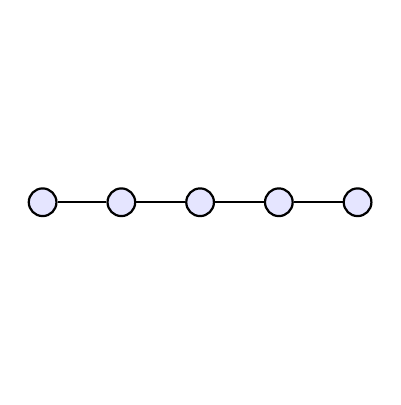
\begin{tikzpicture}[thick,main node/.style={circle,fill=blue!10,draw,minimum size=10pt}]
  	\node[main node] at (0,0) (1) {};
  	\node[main node] at (1,0) (2) {};
  	\node[main node] at (2,0) (3) {};
  	\node[main node] at (3,0) (4) {};
  	\node[main node] at (4,0) (5) {};
  	
  	\node[] at (0,-2.1) {};
  	\node[] at (0,2.1) {};
  	
  	
  	\path[-,every node/.style={font=\sffamily\Large}]
  	(1) edge node[left] {} (2)
  	(2) edge node[left] {} (3)
  	(3) edge node[left] {} (4)
  	(4) edge node[left] {} (5);
\end{tikzpicture}
}
\subfigure[Étoile]{
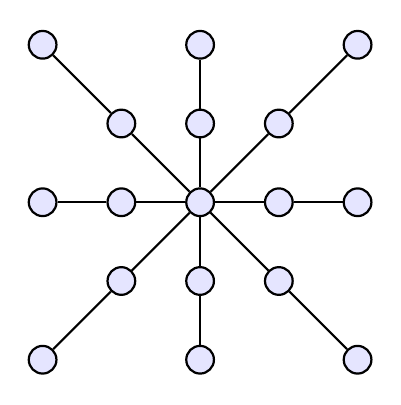
\begin{tikzpicture}[thick,main node/.style={circle,fill=blue!10,draw,minimum size=10pt}]
  	\node[main node] at (0,0) (1) {};
  	\node[main node] at (1,0) (2) {};
  	\node[main node] at (2,0) (3) {};
  	\node[main node] at (3,0) (4) {};
  	\node[main node] at (4,0) (5) {};
  	
  	\node[main node] at (2,1) (6) {};
  	\node[main node] at (2,2) (7) {};
  	
  	\node[main node] at (2,-1) (8) {};
  	\node[main node] at (2,-2) (9) {};
  	
  	\node[main node] at (1,1) (10) {};
  	\node[main node] at (0,2) (11) {};
  	
  	\node[main node] at (1,-1) (12) {};
  	\node[main node] at (0,-2) (13) {};  
  	
  	\node[main node] at (3,1) (14) {};
  	\node[main node] at (4,2) (15) {};
  	
  	\node[main node] at (3,-1) (16) {};
  	\node[main node] at (4,-2) (17) {};    		
  	
  	\node[] at (0,-2.1) {};
  	\node[] at (0,2.1) {};
  	
  	\path[-,every node/.style={font=\sffamily\Large}]
  	(1) edge node[left] {} (2)
  	(2) edge node[left] {} (3)
  	(3) edge node[left] {} (4)
  	(4) edge node[left] {} (5)
  	
  	(3) edge node[left] {} (6)
  	(6) edge node[left] {} (7)
  	
  	(3) edge node[left] {} (8)
  	(8) edge node[left] {} (9)
  	
  	(3) edge node[left] {} (10)
  	(10) edge node[left] {} (11)
  	
  	(3) edge node[left] {} (12)
  	(12) edge node[left] {} (13)  	
 
   	(3) edge node[left] {} (14)
  	(14) edge node[left] {} (15) 
  	
  	(3) edge node[left] {} (16)
  	(16) edge node[left] {} (17);
\end{tikzpicture}
}
\subfigure[Arbre]{
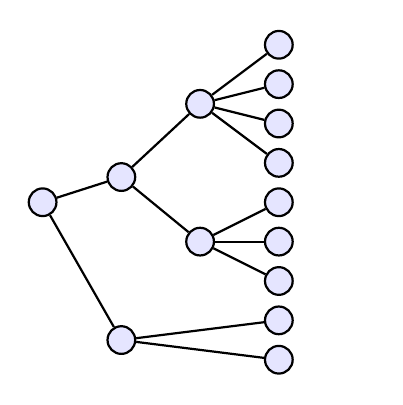
\begin{tikzpicture}[thick,main node/.style={circle,fill=blue!10,draw,minimum size=10pt}]
  	
  	\node[main node] at (0,0) (0) {};
  	\node[main node] at (1,0.32) (10) {};
  	\node[main node] at (1,-1.75) (11) {};
  	\node[main node] at (2,1.25) (20) {};
  	\node[main node] at (2,-0.5) (21) {};
  	\node[main node] at (3,2) (30) {};
  	\node[main node] at (3,1.5) (31) {};
  	\node[main node] at (3,1) (32) {};
  	\node[main node] at (3,0.5) (33) {};
  	\node[main node] at (3,0) (34) {};
  	\node[main node] at (3,-0.5) (35) {};
  	\node[main node] at (3,-1) (36) {};
  	\node[main node] at (3,-1.5) (37) {};
  	\node[main node] at (3,-2) (38) {};
  	
  	\node[] at (0,2.1) {};
  	\node[] at (4.1,-2.1) {};  	
  	
  	\path[-,every node/.style={font=\sffamily\Large}]
  	(0) edge node[left] {} (10)
  	(0) edge node[left] {} (11)
  	(10) edge node[left] {} (20)
  	(10) edge node[left] {} (21)
  	(11) edge node[left] {} (37)
  	(11) edge node[left] {} (38)
  	(20) edge node[left] {} (30)
  	(20) edge node[left] {} (31)
  	(20) edge node[left] {} (32)
  	(20) edge node[left] {} (33)
  	(21) edge node[left] {} (34)
  	(21) edge node[left] {} (35)
  	(21) edge node[left] {} (36);
\end{tikzpicture}
}
\subfigure[Boucle simple]{
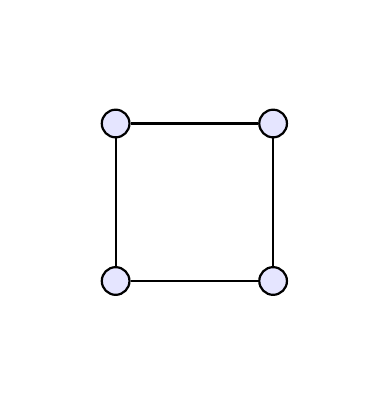
\begin{tikzpicture}[thick,main node/.style={circle,fill=blue!10,draw,minimum size=10pt}]
  	
  	\node[main node] at (1,1) (1) {};
  	\node[main node] at (1,-1) (2) {};
  	\node[main node] at (3,-1) (3) {};
  	\node[main node] at (3,1) (4) {};
  	
  	\node[] at (0,-2.1) {};
  	\node[] at (4,2.1) {};
  	
  	\path[-,every node/.style={font=\sffamily\Large}]
  	(1) edge node[left] {} (2)
  	(2) edge node[left] {} (3)
  	(3) edge node[left] {} (4)
  	(4) edge node[left] {} (1);
\end{tikzpicture}
}
\subfigure[Grille 2D]{
\begin{tikzpicture}[thick,main node/.style={circle,fill=blue!10,draw,minimum size=10pt}]
	\foreach \i in {0,...,4}{
		\pgfmathtruncatemacro{\x}{\i-2}
		\pgfmathtruncatemacro{\a}{\i-1}
		\foreach \j in {0,...,4}{
			\pgfmathtruncatemacro{\y}{\j-2}
			\pgfmathtruncatemacro{\b}{\j-1}
			
			\node[main node] at (\i,\j) (\i\j) {};
			
			\ifthenelse{\i>0}{
				\path[-] (\a\j) edge node[left] {} (\i\j);
			}
			
			\ifthenelse{\j>0}{
				\path[-] (\i\b) edge node[left] {} (\i\j);
			}			
		}
	}
\end{tikzpicture}
}
\subfigure[Connexité complète]{
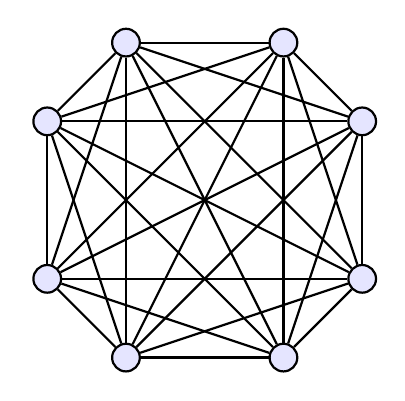
\begin{tikzpicture}[thick,main node/.style={circle,fill=blue!10,draw,minimum size=10pt}]
	\node[main node] at (0,1) (0) {};
	\node[main node] at (1,2) (1) {};
	\node[main node] at (3,2) (2) {};
	\node[main node] at (4,1) (3) {};
	\node[main node] at (4,-1) (4) {};
	\node[main node] at (3,-2) (5) {};
	\node[main node] at (1,-2) (6) {};
	\node[main node] at (0,-1) (7) {};
	
	
	\foreach \i in {0,...,6}{
		\foreach \j in {\i,...,7}{
			\path[-] (\i) edge node[left] {} (\j);
		}
	}
	
\end{tikzpicture}
}

\caption{Illustration de graphes acycliques sur la première ligne et de graphes avec cycle sur la seconde ligne. Seuls les problèmes qui s'écrivent sous la forme d'un graphe acyclique peuvent être traités par DP}
\label{fig:tree_ex}
\end{figure}

\subsubsection{Optimisation d'un graphe acyclique par propagation de croyance (BP)}

La propagation de croyance (BP) peut être utilisée pour estimer le MAP d'une chaîne de Markov 1D. Un message $m_{p \rightarrow q}$ est associé à tout arc $(\mathcal{V}_p,\mathcal{V}_q)$ du graphe. Les messages sont initialisée et mis à jour à l'aide de la règle de mise à jour
\begin{equation}
m_{p \rightarrow q}(k) \leftarrow \min_{k}{Data_p(k) + Reg_{pq}(k,d_q) + \sum_{(t,p) \in \mathcal{E}, k \neq q} m_{t \rightarrow p}(k)}
\end{equation}
Les message sont initialés et mis à jour dans un certain ordre. Il existe de nombreuse variante qui résident dans l'initialisation, dans heuristique du choix de les variables à mettre à jour. Cette méthode converge vers le minimum global sur un graphe acyclique. Dans le cas d'une chaîne 1D, appliquer la BP en mettant jour les messages dans l'ordre dans les deux sens est équivalent à la méthode présentée dans la Partie~\ref{sss:min_DP}. Dans le cas plus générale où la chaîne est acyclique, l'arbre qui représente cette chaîne peut être optimiser globalement en deux passes. La première passe en parcourant le graphe de la racine vers les feuilles puis des feuilles vers la racine.

\subsubsection{Décomposition en chaînes acycliques}

Dans le cas où le graphe possède des cycles, son optimisation devient $NP$ difficile. Des méthodes permettent de résoudre le problème de manière approchée. Certaines consistent à approcher la chaînes complexe par un arbre en élaguant le graphe. C'est le cas de SGM décrit dans la Partie~\ref{ss:SGM} ci-après et de TRW. La BP généralisée peuvent être appliquée, il s'agit de mettre à jour les message comme dans la méthode BP classique, toutefois la présence de cycle peut empêcher l'algorithme de converger. Des heuristique sont mis en ouvre pour corriger en partie des effets.

\subsection{Appariement semi-global (SGM)}
\label{ss:SGM}

\begin{figure}
\centering
%\subfigure[4 Directions]{\myimage{4}{0}{0}}
%\subfigure[8 Directions]{\myimage{4}{0}{1}}
%\subfigure[16 Directions]{\myimage{4}{1}{1}}
\caption{Chemins pris en compte dans l'étape d'agrégation de SGM pour un pixel donnée (en \color{red} rouge \color{black}) pour $4$,$8$ et $16$ directions. Les pixels prise en compte, $\boldsymbol{\chi}^{\boldsymbol{r}}_p$ sont représentés en bleu-vert. Plus le nombre de direction est grand, plus la couverture de l'image est grande.}
\label{fig:SGM_16}
\end{figure}

La détermination d'une carte de profondeur est le plus souvent formulée par l'optimisation d'un grille 2D. Ce problème ne peut donc pas être résolue par la méthode présenté précédemment. Une approche est le limiter le problème à un problème 1D.
	\begin{equation}
	\label{eq:Emulti_1D_1}
	E^{\boldsymbol{C}}(\boldsymbol{l}) = \sum_{p \in \boldsymbol{I} \cap \boldsymbol{C}} D_p(l_p) +  \sum_{(p,q) \in \boldsymbol{N'} \cap \boldsymbol{C}^2} R_{pq}(l_p,l_q)
	\end{equation}
	où $C$ est un ensemble de pixel formant un chemin 1D. Une solution est résoudre indépendamment les lignes de l'image. L'inconvénient de cette approche est qu'aucune information n'est partagée entre les lignes et cohérence verticale de la solution n'est pas garanti donnant lieu à des artefact dans la solution. La solution par résolution indépendante  des lignes ou des colonnes est donnée Figure~\ref{fig:SGM0}.

\begin{figure}
\centering
\includegraphics[scale=0.4]{Images/3_SGM0}
\includegraphics[scale=0.4]{Images/3_SGM1}
\caption{Carte de disparité obtenu par selon les lignes à gauche et selon les colonnes à droite. Le modèle est une attache au données norme L2 tronqué au-delà de la valeur 18 et la régularisation un fonction $P1_P2$ de paramètre $(60,600)$.}
\label{fig:SGM0}
\end{figure}	
	
\subsubsection{La méthode SGM}
	
La méthode $SGM$, proposé par \cite{Hirschmuller08PAMI}, consiste à ne pas seulement prendre en compte l'information d'un chemin 1D, mais de plusieurs chemins 1D formant une étoile autour du pixel considéré. Soit $\boldsymbol{r}$ un ensemble de direction dans l'image, si $r \in \boldsymbol{r}$ alors  $-r \in \boldsymbol{r}$, de sorte que toutes les directions viennent par couple. La solution du problème est définie comme
\begin{equation}
\begin{aligned}
l^{SGM}_p &= \argmin_{l}{SGM(p,l)} \\
l^{SGM}_p &= \argmin_{l}{ Data_i(l) + \sum_{r \in \boldsymbol{r}}{Acc_{r}(p,l)}}  \\
&= \argmin_{l}{\min_{\boldsymbol{l}|l_p=l}E^{\boldsymbol{\chi}^{\boldsymbol{r}}_p}(\boldsymbol{l})}
\end{aligned}
\end{equation}
où $Acc_{r}$ est l'accumulation dans la direction $r$, $\boldsymbol{\chi}^{\boldsymbol{r}}_p$ l'ensemble des pixels dans les directions $\boldsymbol{r}$ par rapport à $p$. Les pixels de $\boldsymbol{\chi}^{\boldsymbol{r}}_p$ sont représentés en bleu dans la Figure~\ref{fig:SGM_16} pour 4, 8 et 16 directions par rapport au pixel central.

Dans \citep{Hirschmuller08PAMI}, les coûts calculés sont légèrement différents. Si la position $p$ est en dehors de l'image $L_r(p,l) = \boldsymbol{0}$ et sinon $L_r(p,l)$ est défini de manière récursive en fonction des valeurs obtenu à la position prétendante $L_r(p{-}r,l)$,
\begin{equation}
	L_r(p,l) = D_{p}(l) + \min_{k}{R_{p,p{-}r}(l,k) + L_r(p{-}r,l)} - \min_{k}{L_r(p{-}r,l)}
\end{equation}
Le terme $\min_{k}{L_r(p{-}r,l)}$ est constant, il ne modifie pas la solution du problème mais permet de garder les coûts dans un intervalle. Si $T_D$ majore $D_{p}$ et $T_R$ majore $R_{p,p{-}r}$ alors
\begin{equation}
	L_r(p,l) \leq T_D + T_R
\end{equation}
L’énergie $SGM^{*}$ est définie par pixel,
\begin{equation}
	SGM^{*}(p,l) = \sum_{r}{L_r(p,l)}
\end{equation}
Les coûts $L_r$ sont reliés aux accumulations $Acc_r$ présentés précédemment  par la relation $L_r(p,l)= k_p + Acc_r(p,l) + Data_p(l)$, $k_p$ une constante, ainsi
\begin{equation}
	SGM^{*}(p,l) = K_p + (|r|{-}1)Data_p(l) + SGM(p,l)
\end{equation}
où $K_p$ est une constante et $|r|$ le nombre de direction prise en compte. Les résultats de carte de disparité sont donnés pour 4, 8 et 16 direction dans la Figure~\ref{fig:SGMs}. Lorsque le nombre de direction prise en compte est élevé la couverture de l'image augmente et l’agrégation des coûts devient de plus en plus isotrope. Cela a pour effet de limiter les artefacts sur la solution. Cette augmentation a un coût en terme de calcul, de plus il peut être intéressant dans certains cas de favoriser les directions principales dans l’agrégation des coûts.

\begin{figure}
\centering
\includegraphics[scale=0.4]{Images/3_GC}
\includegraphics[scale=0.4]{Images/3_SGM4}
\includegraphics[scale=0.4]{Images/3_SGM8}
\includegraphics[scale=0.4]{Images/3_SGM16}
\caption{Carte de disparité obtenues gauche à droite, et de haut en bas par coupure de graphe (schéma Alterné-C, une itération) et par méthode SGM en prenant en compte 4, 8 et 16 directions. La modèle est le même que dans la Figure\ref{fig:SGM0}}
\label{fig:SGMs}
\end{figure}

\subsubsection{Méthode semi-globale}

La méthode SGM est qualifiée de semi-globale. Sous certain aspect elle s'apparente aux méthodes globale ou sur d'autre aux méthodes locales. D'une part  sa formulation est une relaxation d'une énergie globale, en ce sens la solution SGM est une approximation de la solution globale. D'autre part, il s'agit d'une méthode de calcul de coût sur un voisinage de pixel. Même si le coût intègre des valeur d'attache aux données et des valeurs de régularisation, les valeurs de l’énergie SGM en chaque pixel sont indépendante, ce qui la rapport des méthodes locales. En outre, SGM est parfois présenté comme une méthode d'agréation des coût plutôt qu'une méthode d'optimisation. L'enjeu de ce positionnement est de savoir comment doit être interprété l’énergie SGM : comme une vraisemblance ou une estimée de la probabilité à priori.

\subsection{Variantes de la méthode}
\label{ss:SGM_variantes}

La méthode SGM consiste à restreindre l'ensemble des pixels mis en jeu et ignorer les pixels en dehors. Cela a pour conséquence que de nombreux liens entre pixels sont pas pris en compte. Il en résulte un écart important entre l’énergie globale de la solution SGM et le minimum global du problème. Prendre en compte plus de lien pour un nombre même nombre de direction permet de réduire cet écart. La règle de récursion peut être modifiée pour prendre en compte l'énergie accumulée dans la direction $r$ et dans la direction $r_{\perp}$, la direction perpendiculaire à $r$ dans le sens direct.

\subsubsection{Variante CAT}

 Dans la méthode $CAT$ \cite{Ha15ICIP}, le coût acculé est le minimum du coût dans les deux directions, 
\begin{equation}
	L_r(p,l) = D_{p}(l) + \min{
  \left\{
      \begin{aligned}
      &  \min_{k}{R_{p,p{-}r}(l,k) + L_{r}(p{-}r,l)} \\
      &  \min_{k}{R_{p,p{-}r_{\perp}}(l,k) + L_{r_{\perp}}(p{-}r_{\perp},l)}  \\
      \end{aligned}
    \right.
    }
    \label{eq:CAT}
\end{equation}
La méthode montrent des améliorations sur les bases d'évaluation, toutefois la justification théorique avancée par les auteurs est erronée. Les auteurs constatent que la construction les coûts calculés dans $CAT$ sont inférieurs à ceux de $SGM$ et en déduisent la même inégalité sur l’énergie globale. Un contre exemple où la solution issue de $SGM$ possède une énergie globale inférieure à l’énergie de la solution $CAT$ est donné dans la Figure~\ref{fig:counter}. En outre comparer en valeur des énergies différentes n'a pas de sens, d'autant plus que CAT est une version moins contrainte de SGM, la baisse en valeur de l'énergie est donc liée à la relaxation du problème et non à une meilleure optimalité de la solution. En analysant le coût $L_r$, nous remarquons qu'il correspond au chemin de coût minimal par déplacement de $r$ ou $r_{perp}$ depuis $p$, de sorte que les plus courts chemins en distance de Manhattan au bord de l'image sont privilégiés.

\begin{figure}
\centering
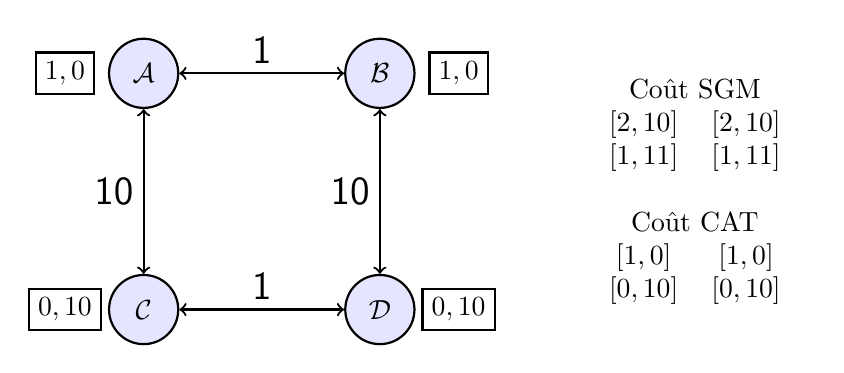
\begin{tikzpicture}[thick,main node/.style={circle,fill=blue!10,draw,minimum size=25pt}]
  	\node[main node] at (-7,1.5) (1) {$\mathcal{A}$};
  	\node[main node] at (-7,-1.5) (2) {$\mathcal{C}$};
  	\node[main node] at (-4,1.5) (3) {$\mathcal{B}$};
  	\node[main node] at (-4,-1.5) (4) {$\mathcal{D}$};
  	
  	\path[<->,every node/.style={font=\sffamily\Large}]
  	(1) edge node[left] {10} (2)
  	(3) edge node[left] {10} (4);
  
  	\path[<->,every node/.style={font=\sffamily\Large}]
  	(1) edge node[above] {1} (3)
  	(2) edge node[above] {1} (4);  
  
  	\node[draw] at (-8,1.5) {$1,0$};
  	\node[draw] at (-8,-1.5) {$0,10$};
  	\node[draw] at (-3, 1.5) {$1,0$};
  	\node[draw] at (-3,-1.5) {$0,10$};
 	
 	 	
    \matrix[ampersand replacement=\&]{
        \node at (8,0) {
            \begin{tabular}{cc}
                \multicolumn{2}{c}{{Coût SGM}} \\
                $[2,10]$ & $[2,10]$ \\
                $[1,11]$ & $[1,11]$ \\
                & \\
                \multicolumn{2}{c}{{Coût CAT}} \\
                $[1,0]$ & $[1,0]$ \\
                $[0,10]$ & $[0,10]$ \\
            \end{tabular}
    }; 
    \\
    };
\end{tikzpicture}
\caption{La figure représente un problème de 4 variables binaires. Les problème est représenté par un graphe dans la fonction pseudo-booléenne correspondante est $f(a,b,c,d)=\bar{a}+\bar{b} + ab + \bar{a}\bar{b} + ab + \bar{c}\bar{d} + 10( c + d + ac + \bar{a}\bar{c} + bd + \bar{b}\bar{d})$. Les coûts obtenues par la méthode SGM et la méthode CAT sont donnés à droite de la figure. Les coût CAT sont inférieur aux coût SGM, néanmoins SGM donne l'affectation $f(0,0,0,0)=2$ et CAT donne l'affectation $f(1,1,0,0)=20$. CAT n'est donc pas nécessairement un meilleur optimiser de l’énergie globale.}
\label{fig:counter}
\end{figure}

Il est à noter que la solution issue de CAT est sensible à une constante ajoutée sur une attache aux données. Cette dernière peut modifier la sélection faite par le minimum selon deux directions. Nous proposons de retrancher une constantes aux coût accumulé de manière analogue à \cite{Hirschmuler}. L'expression (\ref{eq:CAT}) devient
\begin{equation}
	L_r(p,l) = D_{p}(l) + \min{
  \left\{
      \begin{aligned}
      &  \min_{k}{R_{p,p{-}r}(l,k) + L_{r}(p{-}r,l)} - \min_{k}{L_r(p{-}r,l)} \\
      &  \min_{k}{R_{p,p{-}r_{\perp}}(l,k) + L_{r_{\perp}}(p{-}r_{\perp},l)} - \min_{k}{L_{r_{\perp}}(p{-}r,l)} \\
      \end{aligned}
    \right.
    }
\end{equation}
L'interprétation est alors plus difficile, toutefois en considérant que la sélection par le minimum entre les deux directions suit un loi de Bernoulli, la probabilité que le chemin zigzague $k$ fois en $n$ tirage suit une Loi binomiale. Ainsi, les pixels dans la direction de la première diagonale par rapport au pixel courant ont le plus de chance d'être sélectionnés.

\subsubsection{Variante MGM}

Tout comme $CAT$, le $MGM$ proposé par \cite{FaccioloBMVC15} met en jeu deux directions $r$ et $r_{\perp}$ dans la règle de récursion, et sélectionne la moyenne des minimums dans les deux directions. 
\begin{equation}
	L_r(p,l) = D_{p}(l) + \text{moy}{
  \left\{
      \begin{aligned}
      &  \min_{k}{R_{p,p{-}r}(l,k) + L_{r}(p{-}r,l)} \\
      &  \min_{k}{R_{p,p{-}r_{\perp}}(l,k) + L_{r_{\perp}}(p{-}r_{\perp},l)}  \\
      \end{aligned}
    \right.
    }
\end{equation}
La valeur de $C_r$ dépend de tous les pixels compris dans le cadran définit par les vecteurs $-r$ et $-r_{\perp}$. Pour comprendre comment se traduit la modification de la récursion sur l’énergie optimisée, nous définissons la contribution d'un pixel à $p$ à la valeur de $L_r$ évaluée en $p_0$ comme étant la somme des coefficients devant les terme en $D_p$ dans $C_r$ évalué en $p_0$. Un pixel contribue pour moitié à valeur de $L_r$ situé dans les directions $r$ et $r_{\perp}$. Ainsi la contribution d'un pixel à la valeur de $L_r$ suit une loi binomiale
\begin{equation}
	\text{Contribution}(p,p_0) = \frac{1}{2^{v_i + v_j}} \binom{v_i + v_j}{v_i}
\end{equation}
avec $(v_i,v_j)$ les coordonnées du vecteur entre $p$ et $p_0$ dans la base $(r,r_{\perp})$, ces coordonnées sont positives. Ainsi les contributions à distance de Manhattan somment à 1 et décroissent en s’éloignant de la première diagonale. Plus généralement, les chemin qui "zigzaguent" ont plus l'importance dans le calcul du coût.

schéma, pour une direction $r$ en $SGM$, en variante 1, et en variante 2.


\subsubsection{Proposition de variantes exploitant à l'anisotropie des méthodes}

Nous remarquons que ces deux méthodes défavorisent les chemins droits dans le calcul du coût par rapport aux chemins qui "zigzaguent". Nous proposons de modifier les méthodes $CAT$ et $MGM$ pour exploiter cette anisotropie.

\begin{equation}
	L_r(p,l) = D_{p}(l) + \text{somme}{
  \left\{
      \begin{aligned}
      &  (1-a)\min_{k}{R_{p,p{-}r}(l,k) + L_{r}(p{-}r,l)} \\
      &  a\min_{k}{R_{p,p{-}r_{\perp}}(l,k) + L_{r_{\perp}}(p{-}r_{\perp},l)}  \\
      \end{aligned}
    \right.
    }
\end{equation}


\begin{equation}
	L_r(p,l) = D_{p}(l) + \min{
  \left\{
      \begin{aligned}
      &  \min_{k}{R_{p,p{-}r}(l,k) + L_{r}(p{-}r,l)} - \min_{k}{L_r(p{-}r,l)} \\
      &  K + \min_{k}{R_{p,p{-}r_{\perp}}(l,k) + L_{r_{\perp}}(p{-}r_{\perp},l)} - \min_{k}{L_{r_{\perp}}(p{-}r,l)} \\
      \end{aligned}
    \right.
    }
\end{equation}

\section{Expérimentations}
\label{s:Expe}

Dans le chapitre prétendant, nous avons comparé les méthodes par coupure de graphe sur le problème de dé-bruitage. Dans ce problème, l'attache aux données est monotonique, elle n'est pas ambiguë et possède donc un seul minimum. Le problème de reconstruction stéréoscopique est plus complexe, en effet l'attache aux données n'est pas monotonique : d'une part elle est ambiguë avec de nombreux minima locaux et d'autre part elle est erronée là où le modèle n'est pas valide. En effet, l'hypothèse de la correspondance en intensité entre pixels appareillés n'est pas toujours valide. Dans le cas des occultations par exemple, la valeur d'attache aux données à la disparité vraie, l'attache aux données prend des valeurs  équivalentes à un mauvais appariement. Pour cette raison le problème de reconstruction est plus complexe à optimiser que le problème de dé-bruitage. Nous allons comparer les différentes méthodes d'optimisation du problème de reconstruction stéréoscopique par coupure de graphe (GC). Puis nous comparerons les méthodes par programmation dynamique (DP). Enfin, nous comparerons les deux familles de méthodes entre elles.

\subsection{Les jeux de données}

Le modèle que nous optimisons est de la forme
\begin{equation}
\begin{aligned}
E(\boldsymbol{l}) &= \sum_{i \in \boldsymbol{I}}{ f( I^g(i,j) - I^g(i-l_i,j) )} + 
\lambda \sum_{(i,j) \in \boldsymbol{N'}}{ g(l_i-l_j) }
\end{aligned}
\end{equation}
Cela correspond à une détermination de carte de profondeur sans contrainte. Il n'y a pas de prise en compte explicite des occultations.

\subsubsection{Middleburry}

La base de test Middleburry est une collection de couple stéréoscopique. Elle présente la particularité de représenter des scènes d'intérieurs dont les conditions d’illumination sont bien maîtrisé. Les couples sont fournies dans la géométrie épipolaire avec la disparité zéro pour les objets les plus éloignés. Pour chaque couple, les vérités de carte disparité est fournie dans les deux points de vue du couple. Cette base a été enrichie d'année en année avec des images de plus en plus complexes.

Du fait de la bonne maîtrise de la prise de vue et d'une bonne calibration des caméras, la correspondance en couleur entre les points homologues est très bonne. Nous n'observons pas d'un écart ou un gain entre les caméras. Les défauts de correspondance viennent principalement de surface non lambertienne qui changent d'aspect entre les points de vue.

% TODO
métrique d’évaluation
citer la base
exemple de couple utilisé par la suite.
histogramme des écarts

Modèle utilisé

Image Tsukuba

\subsubsection{Kitti}

La base de données KITTI est composée de données issues d'un véhicule acquisition mobile. Nous nous intéressons à la partie stéréoscopie de cette base. Il s'agit de couple stéréoscopique de scène routière en géométrie épipolaire. La disparité 0 correspond aux objets à l'infini. Il existe trois réalisations de la base millésimée 2009, 2012, 2015, appelée KITTI09, KITTI12 et KITTI15.
%La base KITTI09 n'est plus disponible.

La base KITTI12 est composée d'un jeu d'apprentissage et d'un jeu de test. Le jeu d'apprentissage est composée des images d'intensité gauche et droite, de deux vérités de cartes de profondeur : la carte 'occ' dite occulté composée de tous les points et la carte 'non-oc' dite "non occultée" limitée au points qui se projette dans l'image droite. Ces cartes sont obtenue par méthodes lidar et sont peu dense. la correspondance en intensité des points homologue est relativement mauvaise.

\begin{figure}
\centering
\includegraphics[scale=0.24]{Images/3_000011_10l}
\includegraphics[scale=1.2]{Images/3_000011_10l_d1}
\hspace{10 px}
\includegraphics[scale=0.24]{Images/3_000011_10r}
\caption{Couple d'image de la base KITTI2105.}
\end{figure}

la base KITTI15 possède des informations supplémentaire. Les images sont fournie en couleur. Les vérité terrain sont données dans la géométrie gauche et droite. A la différence de la base Middleburry la correspondance en couleur entre les points homologues est assez mauvaises. Cela vient de problème d’étalonnage des canaux couleur, ainsi nous préférons travailler sur les intensités.

Conditions d'extérieurs (réflexion sur la route, sur la vitre de la voiture). Les scènes reste simples, mis à part les objets fins du mobilier urbain. Attache aux données robuste

\begin{figure}
\centering
\includegraphics[scale=0.3]{Images/3_e1_000007}
\includegraphics[scale=0.3]{Images/3_e2_000007}
\includegraphics[scale=0.3]{Images/3_e0_000007}
\caption{Exemple d'un couple d'image et de l'écart d'intensité entre les pixels de l'image gauche et de l'image droite pour un appariement à la disparité gauche vraie. Les écarts inférieurs à 5, inférieurs à 10 et supérieurs à 10 sont représentés respectivement en bleu, vert et rouge. Une large proportions des pixels sont dans la dernière catégorie. Cela rend difficile une approche d'appariement par pixel. Dans cette image, ils correspondent principalement à une différence d'éclairement sur la route. De plus une large proportion des pixels avec un écart inférieur à 5 se trouve dans une zone d'ombre. Ainsi, la faiblesse des écarts peut être expliquée en grande partie par la faible dynamique de l'image qui constitue aussi une difficulté pour l'appariement.}
\end{figure}

\subsection{Coupure de graphe}

Dans le cas de la régularisation par la norme $L1$, le problème peut être résolu exactement par la méthode d'Ishikawa. Dans le cadre du dé-buitage nous avons pu constater que l'algorithme $\alpha$-Expansion convergeait vers le minimum global en une itération lorsque l'attache au donnée étaient convexe. Avec une attache au données monotonique mais non-convexe, la solution d'$\alpha$-Expansion s'écarte légèrement du minimum globale et nécessite plus d'itérations pour converger. Dans le cas de la reconstruction stéréoscopique, l'attache au données n'est pas monotonique. Elle est ambiguë et partiellement entachées d'une erreur de modélisation, ce qui devrait impacter les performances des méthodes approchées. En effet, l'énergie possède de très nombreux minima locaux sur lesquels peut s’arrêter l'optimisation. L'initialisation de la solution est plus difficile que pour le dé-bruitage. En effet, il simple maximum de vraisemblance par pixel ne permet pas d'obtenue une solution approchée. Dans les expérimentations, la carte de disparité est initialisée par sélection du ML par bloc de 11 par 11.


\subsection{Cas de la régularisation par la norme L1}

Dans le cas de la régularisation par la norme L1 nous comparant le méthode exacte d'Ishikawa avec les méthodes approchées par fusions binaires. Le modèle d'attache aux données est une fonction quadratique de la différence d'intensité tronquée au delà de la valeur 18. Les résultats pour 4 images test sont données dans la Table~\ref{tab:stereo_L1}. Quatre schémas d'optimisation sont testés ($\alpha$-Expansion, Alterné-C, Alterné-L, Alterné-LQ, cf. Partie TODO). Les sch"mas sont optimisées par trois méthodes (fusion relaxée, QPBO et QPBO-I).

Tout d'abord, la méthode d'optimisation n'a pas un impact en t


\subsubsection{Influence des schémas d'optimisation}

Les méthodes par coupure de graphe arrive à s'approcher du minimum global.

\subsubsection{Influence des méthodes d'optimisation des schémas}

minime, mais influence en temps de convergence.
La durée d'un cycle est plus courte.
Énergie à temps égal ?

\subsubsection{Influence des méthodes d'optimisation}

Attache aux données : L2 tronquée, L1

Dans les cas des méthodes itératives, la carte de disparité est initialisé par sélection du ML par bloc de 11 par 11. 

\begin{table}
\centering
\begin{tabular}{c|ccc|ccc}
 & Énergie & temps & err.KITTI   & Énergie & temps & err.KITTI \\
Méthode &  \multicolumn{3}{c|}{Tsukuba}   & \multicolumn{3}{c}{Venus} \\
\hline
Ishikawa &  \\
$\alpha$-Expansion &  \\
Alterné-C &  \\
Alterné-L &  \\
Alterné-LQ &  \\
Méthode &  \multicolumn{3}{c|}{Cones}   & \multicolumn{3}{c}{Teddy} \\
\hline
Ishikawa &  \\
$\alpha$-Expansion &  \\
Alterné-C &  \\
Alterné-L &  \\
Alterné-LQ &  \\
\end{tabular}
\end{table}







\begin{table}
\begin{tabular}{c|ccc|ccc|ccc}
 &  \multicolumn{3}{c|}{relaxé}   & \multicolumn{3}{c}{QPBO} & \multicolumn{3}{|c}{QPBO-P} \\
 & $\Delta$E & $\tau$t & err   & $\Delta$E & $\tau$t & err & $\Delta$E & $\tau$t & err \\
\hline
\multirow{2}{*}{Schéma} & \multicolumn{9}{c}{Tsukuba} \\
 & \multicolumn{9}{c}{Ishiwaka : $E=\num{6782506}$, $t=2,91$, $err=4,85\%$} \\
\hline
$\alpha$-Exp & \num{15931}   &  133\% &  4,72\% & \num{16030 } &  168\% & 4,70\%  & \num{16030 } & 390\% & 4,70\%  \\
Alt-C & \num{11980}   &  251\% &  4,71\% & \num{12257 } &  312\% & 4,71\%  & \num{12257 } & 732\% & 4,71\%  \\
Alt-L & \num{15674}   &  147\% &  4,70\% & \num{15951 } &  187\% & 4,70\%  & \num{15951 } & 439\% & 4,70\%  \\
Alt-LQ & \num{114862}  &   79\% &  5,11\% & \num{116612} &  103\% & 5,15\%  & \num{116612} & 236\% & 5,15\%  \\
\hline
\multirow{2}{*}{Schéma} & \multicolumn{9}{c}{Venus} \\
 & \multicolumn{9}{c}{Ishiwaka : $E=\num{15110377}$, $t=12,28$, $err=4,21\%$} \\
\hline
$\alpha$-Exp & \num{11668}   &  77\%  &  4,25\% & \num{11996}  & 97 \% & 4,25\%   & \num{11996}  & 203\% & 4,25\%  \\
Alt-C & \num{11364}   & 179\%  &  4,25\% & \num{11972}  & 167\% & 4,26\%   & \num{11972}  & 344\% & 4,26\%  \\
Alt-L & \num{11359}   &  73\%  &  4,25\% & \num{11967}  & 73 \% & 4,26\%   & \num{11967}  & 152\% & 4,26\%  \\
Alt-LQ & \num{34518}   &  42\%  &  4,24\% & \num{31765}  & 54 \% & 4,25\%   & \num{31765}  & 119\% & 4,25\%  \\     
\hline
\multirow{2}{*}{Schéma} & \multicolumn{9}{c}{Cones} \\
 & \multicolumn{9}{c}{Ishiwaka : $E=\num{34098392}$, $t=26,44$, $err=15,28\%$} \\
\hline
$\alpha$-Exp & \num{155233}  &  97\%  & 15,28\% & \num{154558} &  126\% & 15,27\% & \num{154558} & 275\% & 15,27\% \\
Alt-C & \num{153161}  & 200\%  & 15,24\% & \num{152598} &  302\% & 15,26\% & \num{152598} & 682\% & 15,26\% \\
Alt-L & \num{154753}  &  95\%  & 15,24\% & \num{153803} &  127\% & 15,25\% & \num{153803} & 272\% & 15,25\% \\
Alt-LQ & \num{265230}  &  37\%  & 15,32\% & \num{260205} &   49\% & 15,31\% & \num{260205} & 112\% & 15,31\% \\
\hline
\multirow{2}{*}{Schéma} & \multicolumn{9}{c}{Teddy} \\
 & \multicolumn{9}{c}{Ishiwaka : $E=\num{26069743}$, $t=31,78$, $err=17,05\%$} \\
\hline
$\alpha$-Exp & \num{310580}  &  78\%  & 19,04\% & \num{295168} &  101\% & 19,02\% & \num{295168} & 219\% & 19,02\% \\
Alt-C & \num{296612}  & 174\%  & 18,84\% & \num{285854} &  228\% & 18,83\% & \num{285854} & 515\% & 18,83\% \\
Alt-L & \num{308173}  &  84\%  & 18,83\% & \num{294117} &  119\% & 18,82\% & \num{294117} & 240\% & 18,82\% \\
Alt-LQ & \num{353542}  &  26\%  & 19,27\% & \num{348217} &   40\% & 19,27\% & \num{348217} &  89\% & 19,27\% \\
\end{tabular}
\caption{Comparaison des énergies, temps de convergence et taux d'erreur pour 4 images, 5 schémas d'optimisation et 3 méthodes d'optimisation. Les valeurs d’énergie sont données en écart à l’énergie minimale ($\Delta$E , le temps de convergence est pourcentage du temps de la méthode d'Ishikawa ($\tau$t). L'erreur est le pourcentage de pixel à plus d'un pixel de disparité dans la disparité vraies (err). Les méthodes d'optimisation et les schémas d'optimisation sont tels que décris dans la Chapitre, le schéma Alt-L est limité aux sauts dans $[-3,3]$ et le schéma Alt-LQ est en plus quantifié d'un facteur 2.}
\label{tab:stereo_L1}
\end{table}

\begin{figure}
\centering
\includegraphics[scale=0.24]{Images/3_Res_2}
\includegraphics[scale=0.24]{Images/3_Res_3}
\includegraphics[scale=0.24]{Images/3_Res_4}
\includegraphics[scale=0.24]{Images/3_Res_5}
\caption{Carte de disparité de Cones pour les itérations 2, 3, 4 et 5. Les changements par rapport à l'itération précédente sont représentés en rouge.}
\end{figure}


\begin{figure}
\centering
\includegraphics[scale=0.3]{Images/3_sobel_Alp}
\includegraphics[scale=0.3]{Images/3_sobel_Ish}
\caption{Carte de disparité de Cones pour les itérations 2, 3, 4 et 5. Les changements par rapport à l'itération précédente sont représentés en rouge.}
\end{figure}


\subsection{Programmation dynamique}

\subsubsection{Comparaison des énergies}

\begin{figure}
\centering
\includegraphics[scale=0.3]{Images/3_Ex_ML}
\includegraphics[scale=0.3]{Images/3_Ex_SGM4}
\includegraphics[scale=0.3]{Images/3_Ex_SGM8}
\includegraphics[scale=0.3]{Images/3_Ex_SGM16}
\includegraphics[scale=0.3]{Images/3_Ex_Alt}
\caption{Carte de disparité de la paire 199 de la base KITTI2015. Les résultats sont données de haut en bas par énergie globale à 4-connexité décroissante. Les méthodes sont de haut en bas, ML par bloc 11 par 11, SGM4, SGM8, SGM16 et Alterné-C après une itération. Les critère chiffrés sont données dans la Table~\ref{tab:3_Ex}.}
\label{fig:3_Ex}
\end{figure}

\begin{table}
\centering
\begin{tabular}{c|cc}
Méthode & Énergie & Erreur KITTI \\
\hline
ML & \num{41105898} & 9.57\% \\
SGM4 & \num{39619052} & 3.15\% \\
SGM8 & \num{37277431} & 3.33\% \\
SGM16 & \num{37263882} & 3.21\% \\
Alterné-C & \num{27030832} & 16.16\% \\
\end{tabular}
\caption{Résultats chiffrés pour la paire 199 de la base KITTI2015. Les solution sont présentées dans la Figure~\ref{fig:3_Ex}.}
\label{tav:3_Ex}
\end{table}


\begin{table}
\centering
\begin{tabular}{c|c|c}
\multirow{2}{*}{Méthode} & \multicolumn{2}{c}{Erreur KITTI} \\
 & $(P1,P2)=(3,75)$ & $(P1,P2)=(20,300)$ \\
\hline
Alterné-C & 3.0\% & 23.17\% \\
SGM4 & 2.88\% & 1.94\% \\
\end{tabular}
\caption{Résultats chiffrés pour la paire 199 de la base KITTI2015. Les paramètres de régularisation sont choisis pour optimiser le critère KITTI respectivement avec Alterné-C et SGM4.}
\label{tav:3_Ex}
\end{table}


\subsection{Comparaison entre GC et SGM}


%\bibliographystyle{unsrt}
\bibliographystyle{apalike-fr}
\bibliography{../bibliography/Bib_3}

%----------------------------------------------------------------------------------------
\end{document}
%----------------------------------------------------------------------------------------
